\section{Results}\label{sec:results}
\begin{table}[t]\centering\footnotesize
\caption{\textbf{Main results, test set} ($r_{\max}=1.2$). Lift time and grip are means over all lifts and do not depend on
$r$; failures are lifts with slip $>5$\,mm out of 200 (40 for B0, B0S). No failure was a drop. Full statistics:
Table~\ref{tab:perr}.}\label{tab:main}
\setlength{\tabcolsep}{3.2pt}
\begin{tabular}{@{}lccccccc@{}}\toprule
 & $T$ (s) & $F/mg$ & \multicolumn{4}{c}{failures at $r=$} & max slip\\
 & & & 1.0 & 1.1 & 1.2 & 1.3 & (mm)\\\midrule
B0 model & 1.000 & 1.009 & 0 & 0 & 0 & 0 & 0.49\\
B0S model + shield & 1.000 & 1.009 & 0 & 0 & 0 & 0 & 0.49\\
B2 residual & 0.372 & 1.276 & 3 & 25 & 32 & 32 & 56.0\\
B4g B2 + grip shield & 0.372 & 1.358 & 0 & 0 & 0 & 0 & 0.12\\
B4t B2 + time shield & 0.420 & 1.276 & 0 & 0 & 0 & 0 & 0.14\\
B5 trained with shield & 0.370 & 1.361 & 0 & 0 & 0 & 0 & 0.11\\\bottomrule
\end{tabular}\end{table}

\subsection{\Q1: How much faster, and at what grip?}
\finding{Every residual variant lifts 2.7$\times$ faster than the model.} B5 cut the lift time by 0.630\,s (95\% CI
0.629--0.630; Holm-corrected Wilcoxon $p<10^{-10}$ at every $r$), from 1.00\,s to 0.37\,s (Table~\ref{tab:main}). All ten
trained policies ended at the same corner of the action space, $a_T\approx-1$ (Table~\ref{tab:perseed}), so the speed gain
is set by our action range, not by the physics; Section~\ref{sec:extended} widens the range.

\finding{Faster lifts need more grip.} Peak acceleration grows as $1/T^2$, so the model's own grip for a 0.37\,s lift is
35\% higher than for a 1\,s lift. B5 gripped $0.352\,mg$ harder than B0 (CI 0.330--0.374). The unshielded residual gripped
less, $+0.267\,mg$ (CI 0.237--0.304), because it set its grip on average 6\% below the model's grip for its own lift time
(range $-11$\% to $+3$\% across lifts; the five seeds chose $\bar a_F$ between $-0.24$ and $-0.38$).

\finding{The lift is a small part of an episode.} The probe took a median of 4.1\,s (7.5 probe steps, range 4--11), so the
0.63\,s saved shortens a whole episode by about 10\%. A faster probe is a larger opportunity than a faster lift.

\subsection{\Q2: Does the residual stay safe as friction drops?}
\finding{No.} B2's grip cut is nearly harmless without a friction drop: 3 of 200 lifts failed at $r=1$, because the
quasi-static model over-predicts the grip needed for short lifts by about 8\% (Table~\ref{tab:val}) and $\Fs$ adds more
margin. Once the rod does start to slide, kinetic friction is too low to stop it. Failures rose to 25, 32 and 32 of 200 at
$r=1.1$, 1.2 and 1.3, with slips up to 56\,mm. Per object, B2 failed at least once on 14 objects where the model never
failed at $r=1.1$, and on 16 at $r=1.2$ and 1.3, never the reverse (Holm-corrected McNemar $p=0.001$ and $p=0.0004$). The
seeds cut differently: at $r=1.2$ the five B2 policies failed 2, 6, 14, 2 and 8 times in 40 lifts. Every shielded method
had zero failures at every $r$.

\finding{The failure has one mechanism.} Figure~\ref{fig:anatomy} traces one failure. At 0.03\,s, well before peak acceleration, the demand
$g+a$ exceeds the static capacity and the rod starts to creep; at 0.09\,s its speed relative to the fingers passes the
2\,cm/s switching threshold, friction drops to its kinetic level, which lies well below the demand, and the rod slides at
up to 0.2\,m/s for 0.17\,s, coming to rest 21\,mm lower only once the palm decelerates. All 14 failures of the worst seed follow the same pattern (Fig.~\ref{fig:gallery}
in the appendix), with final slips of 9 to 25\,mm. With a certified grip, the same lift shows only an elastic oscillation
of $\pm6$\,mm/s and at most 0.8\,mm of transient displacement.

\begin{figure*}[t]\centering
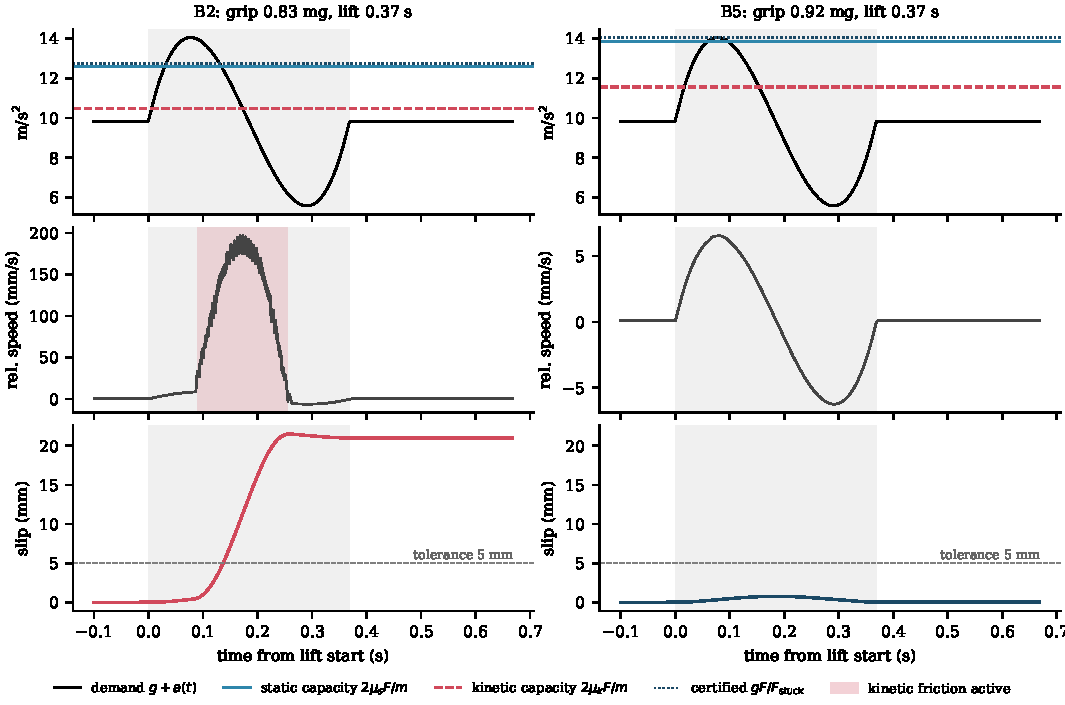
\includegraphics[width=\textwidth]{fig_anatomy.pdf}
\caption{\textbf{Anatomy of a failure} (object 2, $r=1.2$, seed 2). Top: demand $g+a(t)$ against the static, kinetic and
certified capacities for the grip each policy chose. Middle: speed of the fingers relative to the rod, with kinetic friction
active shaded. Bottom: slip. Left, B2: the demand crosses the static capacity at 0.03\,s; the rod breaks away at 0.09\,s,
kinetic friction persists for 0.17\,s, and slip ends at 21\,mm. Right, B5: the certified grip keeps the demand below the static capacity
throughout; the residual motion is elastic and returns to zero.}\label{fig:anatomy}
\end{figure*}

\finding{The result replicates.} On the confirmation set, run once on 40 fresh objects with $r\sim U[1.0,1.3]$, B2 failed
35 of 200 lifts (1, 16 and 18 in the bands $(1,1.1]$, $(1.1,1.2]$ and $(1.2,1.3]$; 15 objects worse than the model, none
better, $p=6\times10^{-5}$), while B4g and B5 failed none at the same speed (0.371\,s and 0.370\,s) and the same extra grip
($+0.32\,mg$) as on the test set (Table~\ref{tab:confirm}).

\begin{figure*}[t]\centering
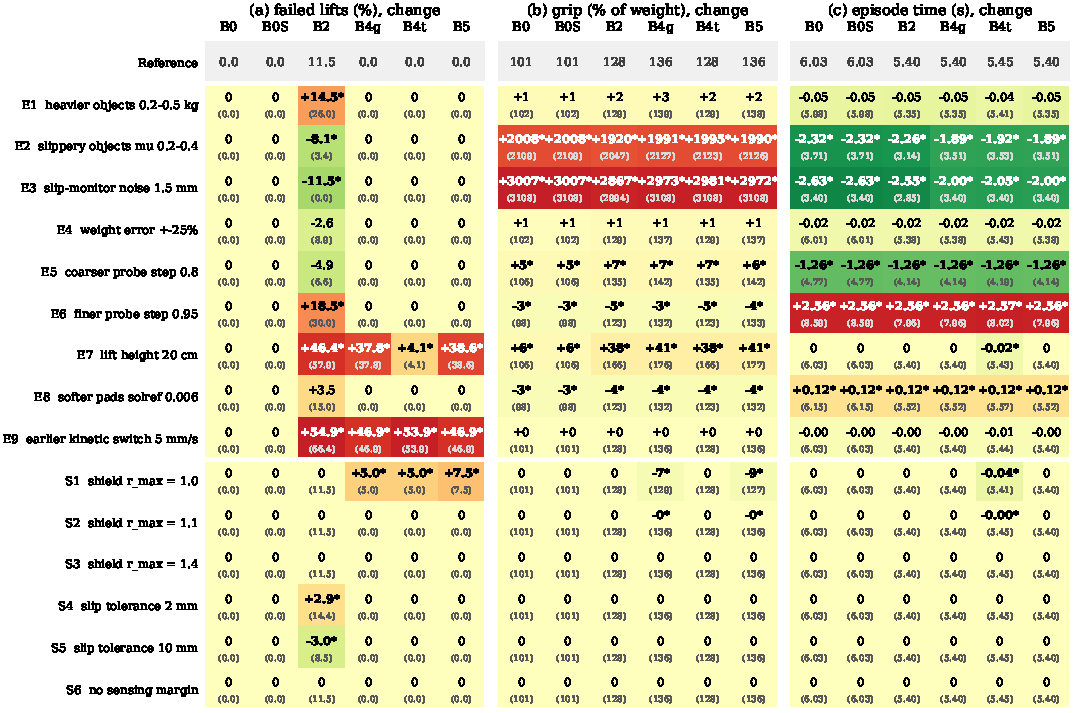
\includegraphics[width=\textwidth]{fig_ctrl_main.pdf}
\caption{\textbf{Controlled study.} Each cell is the change from the reference configuration (top row, absolute values),
with the resulting absolute value in parentheses; * marks a 95\% bootstrap interval that excludes zero. Red is worse
(more failures, more grip, longer episodes). Failures count lifts that slip more than the row's tolerance or drop the rod,
over 160 lifts (B0, B0S) or 800 lifts (learned methods, 5 seeds). Blocks, top to bottom: environment and sensing (E),
shield settings (S), training (T), and diagnostics with the emulator's one-step lag removed (rows ending in L).}\label{fig:ctrl}
\end{figure*}

\subsection{\Q3: Raise the grip, or slow the lift?}
Applied to the same B2 commands, both projections intervened on 95.5\% of lifts and removed every failure
(Table~\ref{tab:main}). \textbf{The grip projection keeps the speed; the time projection keeps the grip.} Grip projection
added 6.4\% grip ($1.358$ vs $1.276\,mg$) at unchanged lift time; time projection kept B2's grip and slowed the lift by
13\% (0.420 vs 0.372\,s). Under our reward, which values one second of lift time like ten object-weights of grip, grip
projection is better. Training with the shield in the loop (B5) gave the same result as adding it at test time (B4g):
0.370 vs 0.372\,s and 1.361 vs 1.358\,$mg$. The shield never declined: a certified command always existed within
30\,N or 2\,s.

\subsection{\Q4: Does the certificate hold, and what does a slip allowance buy?}\label{sec:q4}
\begin{figure*}[t]\centering
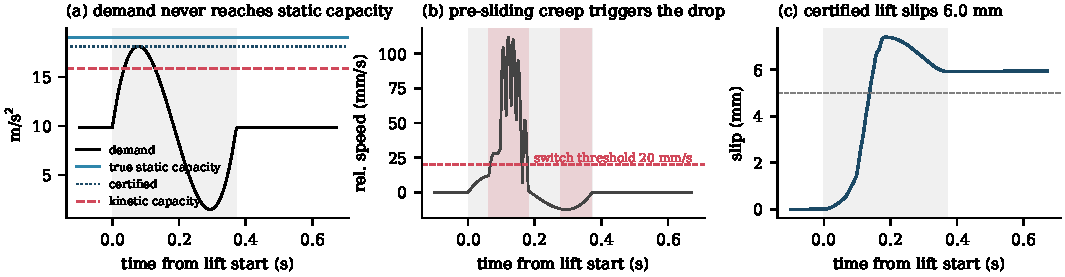
\includegraphics[width=\textwidth]{fig_e7case.pdf}
\caption{\textbf{When the certificate fails} (row E7, lift height 20\,cm, B5, $r=1.2$). (a) The demand peaks at 95\% of the
true static capacity, just below the certified level, so Coulomb friction should hold the rod. (b) The soft contact creeps
at up to 12\,mm/s before peak acceleration; the emulator's kinetic switch, which reads the relative speed with a one-step
lag that adds about 8\,mm/s here, fires at a true relative speed of 12\,mm/s (kinetic friction shaded), and the rod slides. (c) The certified lift ends 6\,mm low.}\label{fig:e7case}
\end{figure*}

\begin{figure*}[t]\centering
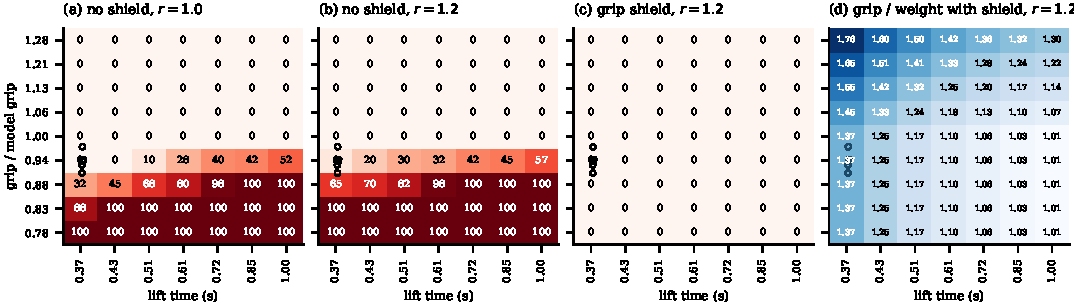
\includegraphics[width=\textwidth]{fig_safetymap.pdf}
\caption{\textbf{Action-space safety map.} Fixed residual actions on the 40 test objects: lift time (columns) against grip
relative to the model's grip for that lift time (rows). (a, b) Percentage of failed lifts without a shield at $r=1.0$ and
$r=1.2$. (c) With the grip shield. (d) Mean grip relative to the object's weight after the shield. Circles mark the mean
effective actions of the five trained B2 policies.}\label{fig:safetymap}
\end{figure*}

\finding{The certificate held wherever its assumption did.} Every certified lift at $r_{\max}=1.2$ had a bound of exactly
zero: the shield placed the grip where slip cannot start. Measured slip was 0.05--0.49\,mm, which is the elastic creep of
Table~\ref{tab:val}, not friction slip. Because any creep exceeds a zero bound, the pre-registered ``exceedance'' rate is
100\% (deviation D1), but the largest excess is a third of the 1.5\,mm margin and no certified lift came within 4.5\,mm of
the tolerance: 0 of 2{,}560 lifts at $r_{\max}=1.2$, including 640 at $r=1.3>r_{\max}$, and 0 of 960 at $r_{\max}=1.4$
(Table~\ref{tab:rmax}). Lifts beyond $r_{\max}$ were safe for a simple reason: slip never started, so the kinetic level never
mattered.

\finding{Assuming friction does not drop is not safe.} With $r_{\max}=1.0$ the shield let B5 grip 6.4\% less
($1.274\,mg$), and 60 of its 600 lifts at $r>1$ slipped more than 5\,mm (10, 25 and 25 at $r=1.1$, 1.2, 1.3; worst excess
over the bound 18\,mm), against 0 of 200 at $r=1$.

\finding{A slip allowance is worth little once friction may drop.} Figure~\ref{fig:teaser}d and Fig.~\ref{fig:bound} explain
why. Allowing 3.5\,mm of slip saves 6.4\% grip if friction does not drop, 4.6\% if it may drop by 2\%, 2.3\% at 5\%,
0.15\% at 10\% and nothing from 15\%. Allowing 10\,mm saves nothing from $r_{\max}=1.2$. Once slip starts, the kinetic
deficit $(g+a)(1-1/r_{\max})$ acts until the palm decelerates, so the certified slip is either zero or large. The ratio of
the certified grip to the no-onset grip was identical for all 40 test objects, because it depends only on $r_{\max}$ and
$T$ (Appendix~\ref{app:cliff}).

\section{Extended Study: What Survives When the Setup Changes?}\label{sec:extended}
The confirmatory study answers \Q1--\Q4 for one configuration. A reader building on it needs to know which conclusions
depend on our choices. We therefore ran a controlled study (overview in Fig.~\ref{fig:overview}, Appendix~\ref{app:ext}): starting from the test-set
configuration, each of 19 rows changes \emph{one} design choice and reruns all six methods on the same 40 objects, four
values of $r$ and the same episode seeds; four rows retrain the residuals. Four diagnostic rows (R0L, E7L, E9L, T2L) were
added after some results were seen, each frozen before it was run. Figure~\ref{fig:ctrl} reports the change in
failure rate, grip and episode time for every cell, with a paired bootstrap over objects marking changes whose 95\%
interval excludes zero (an unpaired bootstrap for E1 and E2, which draw different objects). Table~\ref{tab:changes} in the
appendix describes each change and Table~\ref{tab:controlled} gives absolute values. The study, and the analyses in
Sections~\ref{sec:map}--\ref{sec:tight}, were frozen in a protocol addendum before they were run and are exploratory.





\subsection{Findings that hold}
\finding{The unshielded residual is fragile, and the shield fixes it.} B2's failure rate moved with almost every change:
from 11.5\% in the reference to 26\% for heavier objects (E1), 30\% with a finer probe (E6), 15\% with softer pads (E8) and
14\% with a 2\,mm tolerance (S4). In every one of these rows, and in the weight-error and probe-step rows, B4g, B4t and B5
had zero failures. A finer probe is an instructive case: it brings $\Fs$ closer to the true breakaway grip, which removes
some of the hidden margin that B2 had learned to spend, so B2 fails more while the shielded methods do not notice.

\finding{The cliff holds.} Setting the shield to $r_{\max}=1.1$ (S2) lowered B5's grip by only 0.19 percentage points of the
object's weight, and $r_{\max}=1.4$ (S3) changed nothing: once any drop is assumed, the certified grip is the no-onset grip.
Removing the 1.5\,mm sensing margin (S6) or widening the tolerance to 10\,mm (S5) did not change the shielded grip at all.
Only $r_{\max}=1.0$ (S1) bought grip, $-7$ to $-9$ points, and it cost 5--7.5\% failures, as in \Q4.

\subsection{Findings that break}
\finding{A probe that fails gives the shield nothing to certify.} Our probe starts at the grip that would hold the
estimated weight at $\mu=0.3$. With slippery objects ($\mu_s\in[0.2,0.4]$, E2) the first step already slips for many
objects; with a noisier slip monitor (1.5\,mm, E3) noise alone exceeds the 2.5\,mm motion threshold on the first step. In
both cases the probe reports $\Fs=30$\,N, the maximum grip. The shield then certifies nothing: it declined on 68\% (E2) and
100\% (E3) of lifts and fell back to the slow model lift, at 21 to 31 times the object's weight in grip. This is a safe
failure, but not a gentle one, and Fig.~\ref{fig:ctrl}a shows why failure rates alone mislead here: B2's failure rate
\emph{fell} in these rows because it, too, was handed a crushing grip.

\finding{The certificate assumes friction stays static until gross slip, and that assumption can fail.} Two rows broke the
shield itself. Lifting 20\,cm instead of 10\,cm (E7) doubles the peak acceleration for the same duration; B5 then failed
38.6\% of lifts and B4g 37.8\%, every one with a certified bound of zero. Switching to kinetic friction at 5\,mm/s instead
of 2\,cm/s (E9) gave 46.9\% for both. Figure~\ref{fig:e7case} shows the mechanism. The shield sets the grip at the edge of
onset, where the demand reaches 95\% of the true static capacity at peak acceleration. At that load MuJoCo's soft contact
lets the rod creep relative to the pads, at up to 12\,mm/s in E7 (6.5\,mm/s in the reference). Our emulator decides when
friction drops by comparing the rod's velocity from the previous step with the palm's commanded velocity for the current
step; this one-step lag adds $a\,\Delta t$, about 8\,mm/s at E7's peak acceleration, to the measured relative speed. Creep
plus lag crossed the 20\,mm/s threshold, friction dropped although Coulomb's law says the rod was stuck, and the rod slid.
In the reference configuration the same quantity peaked at 10.8\,mm/s, and no shielded lift ever switched to kinetic
friction (0 of 2{,}560). The time projection was more robust in E7 (4.1\% failures), because a longer lift lowers the peak
demand instead of meeting it at the edge.

\finding{Removing the lag.} (pending)


So E7 was an artefact, but E9 exposes something real. The shield places the grip exactly at the onset boundary, where
the contact already creeps; if friction weakens during that creep, the certificate's premise (static friction until gross
slip) fails. Real contacts also move before they slide: pre-sliding displacement is part of every dynamic friction
model~\cite{canudas1995,olsson1998}, and whether friction weakens during it depends on the materials. \textbf{The practical
fix is a margin on onset}, certifying $g+a\le(1-\delta)\,gF/\Fs$ for some $\delta>0$, which our zero-margin shield did not
have. We report this as found rather than adding the fix after seeing the result.



\subsection{Training choices}\label{sec:trainrows} (pending)

\subsection{An action-space safety map}\label{sec:map}
Why does every policy end up at the fastest lift? We swept fixed residual actions over a $7\times9$ grid of lift times and
grip scales on the 40 test objects (Fig.~\ref{fig:safetymap}). Two facts explain the learned policies. First, \textbf{fast lifts
tolerate grip cuts better}: at the model's grip minus 6\% ($a_F=-0.25$), no lift failed at $T=0.37$\,s with $r=1$, but 52\%
failed at $T=1$\,s. This is the quasi-static conservatism of Table~\ref{tab:val} again: the faster the lift, the more the
model over-predicts the grip it needs, so a policy rewarded for speed and light grip is pushed to the fastest corner, where
the hidden margin is largest. The five B2 policies (circles) sit at that corner, 6--9\% below the model's grip. Second,
\textbf{the margin shrinks once friction may drop}: at $r=1.2$ the same cut failed 8\% of fast lifts and the safe region
receded. With the grip shield, none of the 5{,}040 lifts in the grid failed, and the certified grip (panel d) depends only
on the lift time, as the scale invariance of Appendix~\ref{app:cliff} predicts.



\subsection{How tight is the bound?}\label{sec:tight}
We lifted the 40 test objects with grips 0--15\% below the no-onset grip, at three lift durations and three values of $r$,
and evaluated Proposition~\ref{prop:lift} with $r_{\max}$ equal to the true $r$ (Fig.~\ref{fig:tightness}). Three results
stand out. \textbf{The bound is loose}: among the 1{,}309 lifts with a non-zero bound in which the rod stayed in the grasp,
the median ratio of measured slip to bound was 0.023 (90th percentile 0.50). The probe's 0.9 step and the quasi-static
model's conservatism together leave most under-gripped lifts with little or no slip. \textbf{A zero bound meant no slip}:
the 360 lifts with a zero bound slipped at most 0.49\,mm, all of it creep. \textbf{The bound can be exceeded during long
slides}: 7 lifts, all at $T=1$\,s, $r=1$ and 3\% below the no-onset grip, slipped 26--44\,mm against a bound of 25\,mm. With
$r=1$ no friction switch is involved, so these slides expose a gap between the Coulomb model behind the bound and MuJoCo's
regularised sliding friction~\cite{todorov2012}. They do not affect the shield, which never certifies bounds of this size,
but they mark the limit of what the bound says about a simulated slide that lasts most of a second. The 491 lifts that
dropped the rod all had bounds above 12\,cm.

\begin{figure*}[t]\centering
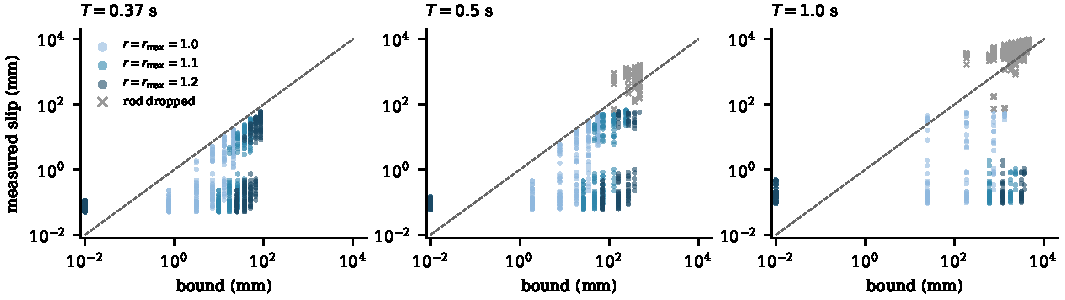
\includegraphics[width=\textwidth]{fig_tightness.pdf}
\caption{\textbf{Bound against measured slip} for deliberately under-gripped lifts (grip 85--100\% of the no-onset grip,
40 objects; log axes, zeros drawn at the left and bottom edges; dashed line: slip equal to the bound). Points below the line
are covered by the bound. Crosses are lifts that dropped the rod, where the slip is the rod's fall.}\label{fig:tightness}
\end{figure*}



